% For LaTeX-Box: root = stat105_F15_exam1B.tex 
%%%%%%%%%%%%%%%%%%%%%%%%%%%%%%%%%%%%%%%%%%%%%%%%%%%%%%%%%%%%%%%%%%%%%%%%%%%%%%%%
%  File Name: stat105_F15_exam1B.tex
%  Purpose:
%
%  Creation Date: 24-09-2015
%  Last Modified: Thu Nov  5 01:12:05 2015
%  Created By:
%%%%%%%%%%%%%%%%%%%%%%%%%%%%%%%%%%%%%%%%%%%%%%%%%%%%%%%%%%%%%%%%%%%%%%%%%%%%%%%%
\documentclass[addpoints]{examsetup}\usepackage[]{graphicx}\usepackage[]{color}
%% maxwidth is the original width if it is less than linewidth
%% otherwise use linewidth (to make sure the graphics do not exceed the margin)
\makeatletter
\def\maxwidth{ %
  \ifdim\Gin@nat@width>\linewidth
    \linewidth
  \else
    \Gin@nat@width
  \fi
}
\makeatother

\definecolor{fgcolor}{rgb}{0.345, 0.345, 0.345}
\newcommand{\hlnum}[1]{\textcolor[rgb]{0.686,0.059,0.569}{#1}}%
\newcommand{\hlstr}[1]{\textcolor[rgb]{0.192,0.494,0.8}{#1}}%
\newcommand{\hlcom}[1]{\textcolor[rgb]{0.678,0.584,0.686}{\textit{#1}}}%
\newcommand{\hlopt}[1]{\textcolor[rgb]{0,0,0}{#1}}%
\newcommand{\hlstd}[1]{\textcolor[rgb]{0.345,0.345,0.345}{#1}}%
\newcommand{\hlkwa}[1]{\textcolor[rgb]{0.161,0.373,0.58}{\textbf{#1}}}%
\newcommand{\hlkwb}[1]{\textcolor[rgb]{0.69,0.353,0.396}{#1}}%
\newcommand{\hlkwc}[1]{\textcolor[rgb]{0.333,0.667,0.333}{#1}}%
\newcommand{\hlkwd}[1]{\textcolor[rgb]{0.737,0.353,0.396}{\textbf{#1}}}%

\usepackage{framed}
\makeatletter
\newenvironment{kframe}{%
 \def\at@end@of@kframe{}%
 \ifinner\ifhmode%
  \def\at@end@of@kframe{\end{minipage}}%
  \begin{minipage}{\columnwidth}%
 \fi\fi%
 \def\FrameCommand##1{\hskip\@totalleftmargin \hskip-\fboxsep
 \colorbox{shadecolor}{##1}\hskip-\fboxsep
     % There is no \\@totalrightmargin, so:
     \hskip-\linewidth \hskip-\@totalleftmargin \hskip\columnwidth}%
 \MakeFramed {\advance\hsize-\width
   \@totalleftmargin\z@ \linewidth\hsize
   \@setminipage}}%
 {\par\unskip\endMakeFramed%
 \at@end@of@kframe}
\makeatother

\definecolor{shadecolor}{rgb}{.97, .97, .97}
\definecolor{messagecolor}{rgb}{0, 0, 0}
\definecolor{warningcolor}{rgb}{1, 0, 1}
\definecolor{errorcolor}{rgb}{1, 0, 0}
\newenvironment{knitrout}{}{} % an empty environment to be redefined in TeX

\usepackage{alltt}

\usepackage{etoolbox}
\usepackage{tikz,pgfplots}
\usepackage{graphicx, fancyhdr}
\usepackage{amsmath, amsfonts}
\usepackage{color}

%% For LaTeX-Box: root = stat105_exam1_info.tex 
%%%%%%%%%%%%%%%%%%%%%%%%%%%%%%%%%%%%%%%%%%%%%%%%%%%%%%%%%%%%%%%%%%%%%%%%%%%%%%%%
%  File Name: stat105_exam1_info.tex
%  Purpose:
%
%  Creation Date: 24-09-2015
%  Last Modified: Thu Sep 24 13:51:36 2015
%  Created By:
%%%%%%%%%%%%%%%%%%%%%%%%%%%%%%%%%%%%%%%%%%%%%%%%%%%%%%%%%%%%%%%%%%%%%%%%%%%%%%%%
\newcommand{\course}[1]{\ifstrempty{#1}{STAT 105}{STAT 105, Section #1}}
\newcommand{\sectionNumber}{B}
\newcommand{\examDate}{October 1, 2015}
\newcommand{\semester}{FALL 2015}
\newcommand{\examNumber}{II}

\newcommand{\examTitle}{Exam \examNumber}

\runningheader{\course{\sectionNumber}}{Exam \examNumber}{\examDate}
\runningfooter{}{}{Page \thepage of \numpages}

\newcommand{\examCoverPage}{
   \begin{coverpages}
   \centering
   {\bfseries\scshape\Huge Exam I \par}
   \vspace{1cm}
   {\bfseries\scshape\LARGE \course{\sectionNumber} \par}
   {\bfseries\scshape\LARGE \semester \par}

   \vspace{2cm}

   \fbox{\fbox{\parbox{5.5in}{\centering 

      \vspace{.25cm} 
      
      {\bfseries\Large Instructions} \\

      \vspace{.5cm} 

      \begin{itemize}
         \item  The exam is scheduled for 80 minutes, from 8:00 to 9:20 AM. At 9:20 AM the exam will end.\\
         \item  A forumula sheet is attached to the end of the exam. Feel free to tear it off.\\
         \item  You may use a calculator during this exam.\\
         \item  Answer the questions in the space provided. If you run out of room, continue on the back of the page. \\
         \item  If you have any questions about, or need clarification on the meaning of an item on this exam, please ask your instructor. No other form of external help is permitted attempting to receive help or provide help to others will be considered cheating.\\
         \item  {\bfseries Do not cheat on this exam.} Academic integrity demands an honest and fair testing environment. Cheating will not be tolerated and will result in an immediate score of 0 on the exam and an incident report will be submitted to the dean's office.\\
      \end{itemize}

   }}}

   \vspace{2cm}

   \makebox[0.6\textwidth]{Name:\enspace\hrulefill}

   \vspace{1cm}

   \makebox[0.6\textwidth]{Student ID:\enspace\hrulefill}
   \end{coverpages}

}


\newcommand{\course}[1]{\ifstrempty{#1}{STAT 105}{STAT 105, Section #1}}
\newcommand{\sectionNumber}{B}
\newcommand{\examDate}{November 5, 2015}
\newcommand{\semester}{FALL 2015}
\newcommand{\examNumber}{II}

%%%%%%%%%%%%%%%%%%%%%%%%%%%%%%%%%%%%%%%%%%%%%%%%%%%%%%%%%%%%%%%%%%%%%%%%%%%%%%%%
\IfFileExists{upquote.sty}{\usepackage{upquote}}{}
\begin{document}

%-- : R code (Code in Document)



\examCoverPage

\begin{questions}

\question

An engineer for City Bikes, a rent-and-return bike company, is working on decreasing the time it takes to bring a bicycle to a complete halt.
The company is interested in fitting bikes with brake that is has consistently short brake times. 
Bike mechanisms are durable and rarely wear out, but the rubber brake pads often do and may be replaced locally (i.e., the type of brake pad used is out of the company's control, but the brand of brake mechanism is within their control).
His goal is to recommend a brake mechanism that has low stopping times regardless of the brake pads used.
He is looking at three different brands of brake mechanism and three common types of rubber brake pads and has decided to use a factorial study to determine which brake mechanism is best.
The engineer assigns the brake mechanism brand to Factor A and the rubber pads to Factor B. 
Stopping speeds for each combination of brake mechanism and brake pads were tested four times under similar condtions.

The results are recorded below.

%-- : R code (Code in Document)


\begin{table}[h]
\centering
\begin{tabular}{lrrr}
   & \multicolumn{3}{c}{Brake Pads} \\
\cline{2-4}
Brand & Type 1 & Type 2 & Type 3\\ \hline \hline
Brand 1 & 8.73 & 8.47 & 9.75 \\
        & 9.16 & 5.72 & 10.93 \\
        & 9.54 & 7.36 & 11.56 \\
        & 8.02 & 5.72 & 12 \\
Brand 2 & 5.36 & 4.53 & 15.01 \\
        & 5.39 & 4.29 & 16.04 \\
        & 5.16 & 4.01 & 14.74 \\
        & 5.26 & 5.85 & 16.24 \\
Brand 3 & 9.2 & 7.52 & 9.15 \\
        & 8.55 & 6.74 & 10.97 \\
        & 8.14 & 6.59 & 10.19 \\
        & 7.49 & 5.22 & 11.98 \\
\hline
\end{tabular}
\end{table}

The following summaries may help in this problem:

%-- : R code (Code in Document)


\begin{table}[h]
\centering
\begin{tabular}{lrrrr}
 & \multicolumn{3}{c}{Brake Pad} \\
\cline{2-4}
Brand   & Type 1                     & Type 2                      & Type 3                       &  \\
\cline{1-4} \cline{1-4}
Brand 1 &                                & $\bar{y}_{12} = 6.82$    & $\bar{y}_{13} = 11.06$   &                                \\
Brand 2 & $\bar{y}_{21} = 5.29$   &                                 & $\bar{y}_{23} = 15.51$   & $\bar{y}_{2 \cdot} = 8.49$ \\
Brand 3 & $\bar{y}_{31} = 8.35$   & $\bar{y}_{32} = 6.52$    & $\bar{y}_{33} = 10.57$   & $\bar{y}_{3 \cdot} = 8.48$ \\
\cline{1-4} 
        & $\bar{y}_{\cdot 1} = 7.5$ &                                 & $\bar{y}_{\cdot 3} = 12.38$   & $\bar{y}_{\cdot \cdot} = 8.63$ \\
\end{tabular}
\end{table}

\begin{parts}

   \part[2] Report the value of $\bar{y}_{1 \cdot}$
   \vspace{2cm}

   \part[2] Report the value of $\bar{y}_{\cdot 2}$
   \vspace{2cm}

   \newpage

   \part[3] Find the fitted main effect of braking using each brand, $a_1$, $a_2$, and $a_3$, that you would get from factorial model that ignores interactions.
   \vspace{3cm}

   \part[3] Ignoring possible interactions, give the estimated values $\hat{y}_{22}$ and $\hat{y}_{23}$.
   \vspace{3cm}

   \part[2] How do the estimated values computed above compare to the average for the same combinations seen in the data? 
            Does it appear that ignoring interactions was a good choice?
   \vspace{2cm}

   \part[5] Using the template below, create a profile plot for this data:

%-- : R plot (results in document)
\begin{knitrout}
\definecolor{shadecolor}{rgb}{0.969, 0.969, 0.969}\color{fgcolor}

{\centering 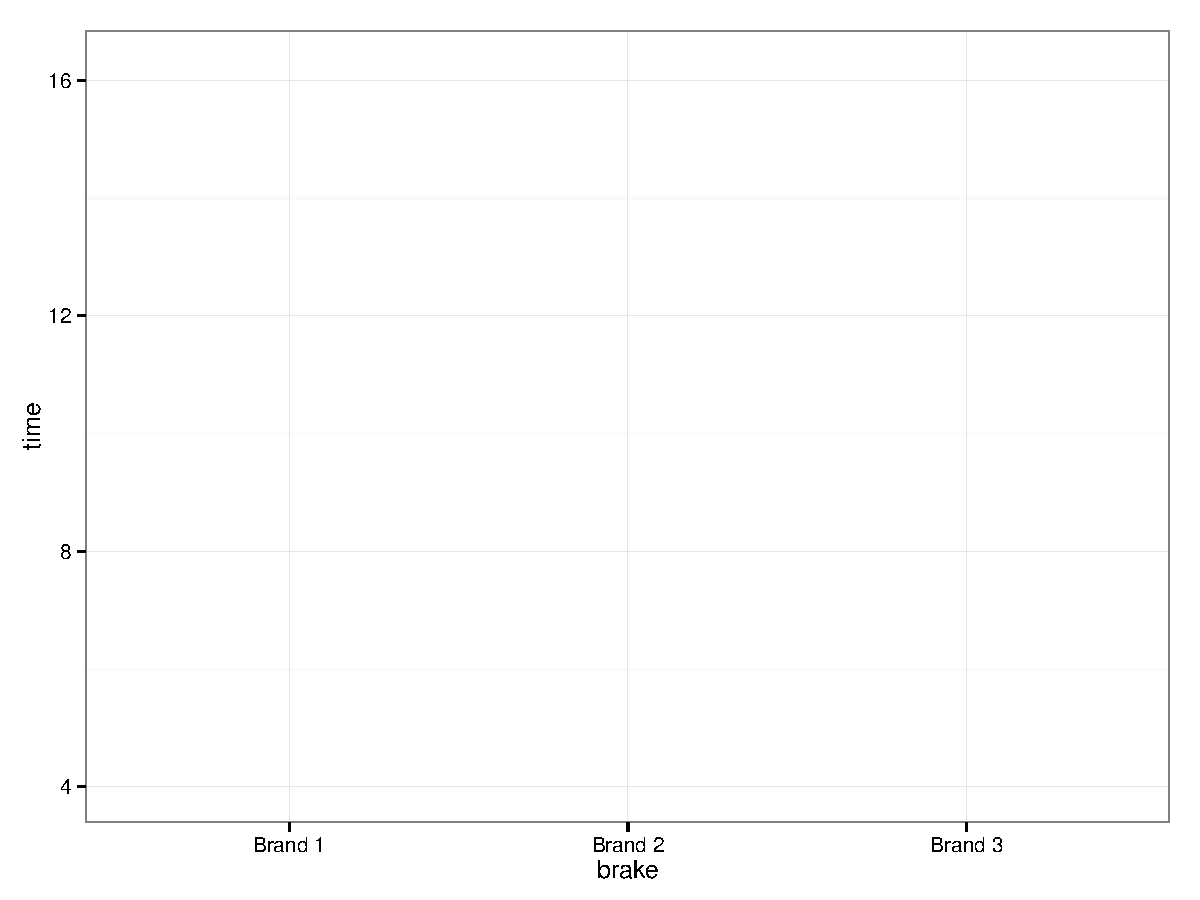
\includegraphics[width=.7\linewidth]{figure/unnamed-chunk-4-1} 

}



\end{knitrout}

   \part[2] Using the plot does it appear that there is an interaction between brake mechanism and rubber type? 
   If you had to recommend a brake mechanism and had to consider low stopping times and consistency across brake pads which would you suggest?
   \vspace{2cm}
\end{parts}

\newpage

\question 


After winning an enormous sum on a (rigged) casino dice game Danny Ocean moves on to another game.
In roullette, a ball bounces on a spinning wheel with 38 pockets numbered 0, 00, 1, 2, ..., 36, and bets are made on which pocket the ball will eventually come to rest. 
In a fair game, the ball has the same chance of coming to a rest in every pocket, but Mr. Ocean has rigged the game (using metallic dust and magnets).
In this rigged version, the ball will come to rest in 00 with probability 0.14, 0 with probability 0.14, and any other of the 36 pockets with probability 0.02.
Mr. Ocean will win his bet if the ball lands in either 00 or 0. 

He defines two random variables: $X$ (which takes the value 1 if he wins the first spin and 0 if he loses), and $T$, the number of attempts needed to win for the first time. \\

\begin{parts}

   \part[2] Provide the probability function for $X$.
   \vspace{2cm} 

   \part[2] Find the variance and expected value of $X$.
   \vspace{2cm} 

   \part[2] Find $\mathbb{E}(T)$. 
   \vspace{2cm}

   \part[2] What is the probability that Danny will win for the first time on his 5th attempt?
   \vspace{3cm}

   \part[4] What is the probability that it will take more than 2 games for Danny to win his first bet?
   \vspace{3cm}

   \part[4] Danny wins, but decides to play five more games - what is the probability that he wins at least one of them?

   \vspace{4cm}

\end{parts}

\newpage

\question

Let $X$ be a normal random variable with a mean of 2 and a varaince of 9 (i.e., $X \sim N(2,9)$) and let $Z$ be a random variable following a standard normal distribution.

\begin{parts}
 \part Find the following probabilities (note: Table B-3 may be helpful):
  \begin{subparts}
     \subpart[2] $P(Z \le 2)$

     \vspace{2cm}

     \subpart[2] $P(|Z| \ge 1)$

     \vspace{2cm}

     \subpart[2] $P(0 \le Z < 3)$

     \vspace{2cm}

     \subpart[2] $P(X < 3)$

     \vspace{2cm}

     \subpart[2] $P(|X| \le 4.5)$

     \vspace{2cm}

  \end{subparts}

  \part[5] Find the value $a$ so that $P(- a + 2 < X < a + 2) = .95$ (approximate as needed).

\end{parts}

\newpage

\question 

Suppose that $X$ is a continuous random variable with probability density function (pdf):
$$
f(x) = 
\begin{cases}
    0 &  x < 0 \\
    c x^2 &  -2  < x < 2 \\
    0 & x \ge 2
\end{cases}
$$
where $c$ is a constant.

\begin{parts}

\part[2] What is the value of $c$ if $f(x)$ is a valid probability density function?

     \vspace{2cm}


\part[5] Sketch the probability density function using the grid below (including the points $(-2, f(2))$ and $(2, f(2))$).

%-- : R plot (results in document)
\begin{knitrout}
\definecolor{shadecolor}{rgb}{0.969, 0.969, 0.969}\color{fgcolor}

{\centering 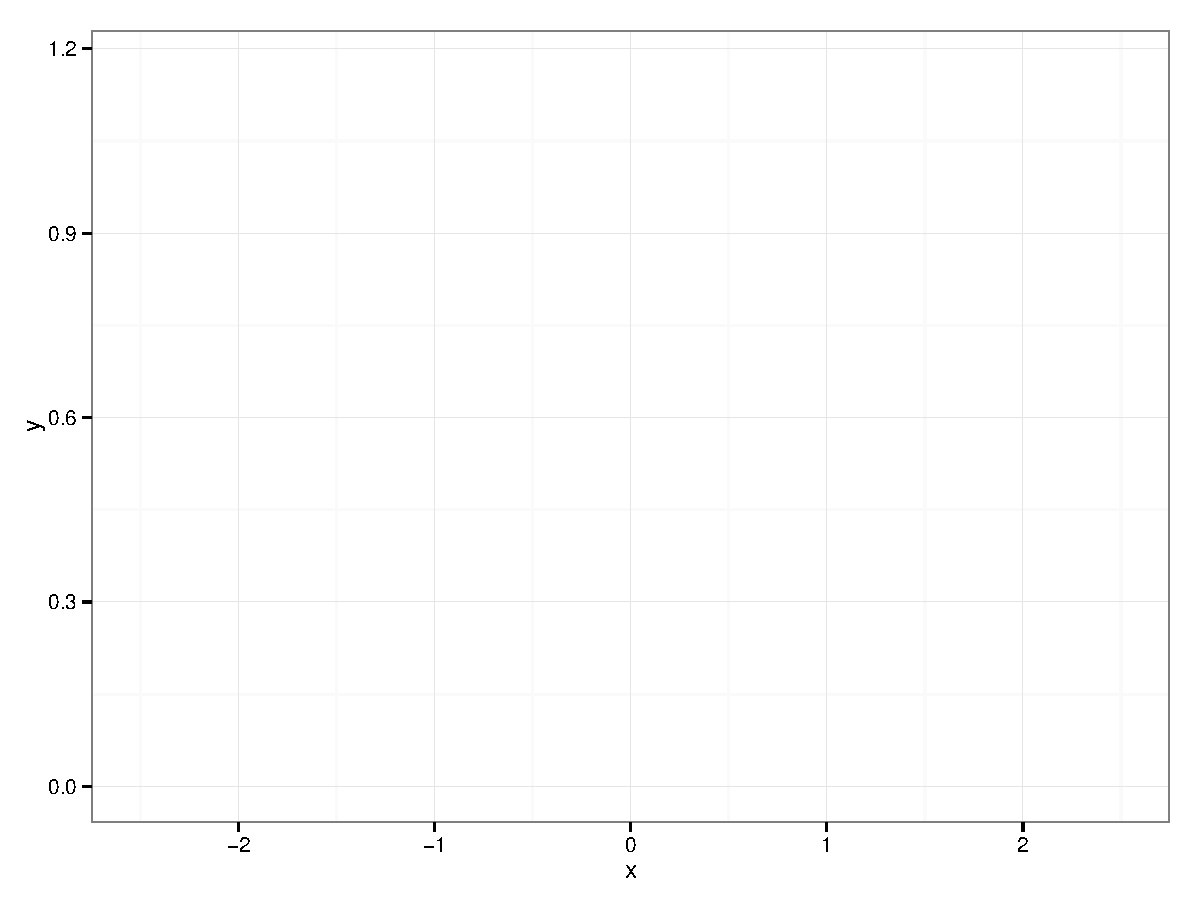
\includegraphics[width=.6\linewidth]{figure/unnamed-chunk-5-1} 

}



\end{knitrout}

\part[4] What is the cumulative density function, $F(x)$?

     \vspace{3cm}

\part[2] What is the probability that $X$ takes a value greater than 1?

     \vspace{2cm}

\part[2] What is the probability that $X$ takes a value between 0 and 1?

     \vspace{2cm}


\end{parts}

\newpage

\question

Suppose we know that $W$ is a binomial random variable with $n = 5$ trials, 
each with the same probability of success $p$, but that the value of $p$ is depends on another random variable $X$.
$X$ will take one of three values, $\frac{1}{4}$, $\frac{2}{4}$, or $\frac{3}{4}$, each with the same probability.
The value $X$ takes will then serve as the value for the probability of success, $p$, for $W$, i.e., if $X = \frac{1}{4}$ then $W$ is a Binomial(5,$\frac{1}{4}$). 
Two of the conditional probability functions that result from this arrangement are below:
$$
f(w|X = \frac{1}{4}) = 
\begin{cases}
   \frac{5!}{(5-w)! w!} (\frac{1}{4})^w (1 - \frac{1}{4})^{5 - w} & w = 0, 1, 2, 3, 4 \text{ or } 5 \\
   0 &  \text{ otherwise }
\end{cases}
f(w|X = \frac{2}{4}) = 
\begin{cases}
   \frac{5!}{(5-w)! w!} (\frac{2}{4})^w (1 - \frac{2}{4})^{5 - w} & w = 0, 1, 2, 3, 4 \text{ or } 5 \\
   0 &  \text{ otherwise }
\end{cases}
$$

In this problem, $f(x,w) = P(X = x, Y = y)$ defines the joint probability function.
\begin{parts}
   \part[2] Find the conditional probability function $f(w | X = \frac{3}{4})$.
   \vspace{2cm}
   \part[2] Find the joint probability $f(\frac{1}{4},0)$.
   \vspace{2cm}
   \part[2] Find the joint probability $f(\frac{2}{4},0)$.
   \vspace{2cm}
   \part[3] Find $f_{W}(0)$.
   \vspace{2cm}
   \part[2] Find $f_{X|W}(\frac{1}{4}|W = 0)$.
   \vspace{2cm}
   \part[2] Find $P(X = \frac{2}{4}|W = 0)$.
   \vspace{2cm}
   \part[2] Find $P(X = \frac{3}{4}|W = 0)$.
   \vspace{2cm}
   \part (\textit{5 bonus points}) If we don't know what value $X$ has taken, but we can observe the value of $W$, what values can $W$ take that would make us believe it is more likely that $X = \frac{2}{4}$ than either of the other two values of $X$?

\end{parts}

\end{questions}

\end{document}
